\documentclass{article}

\usepackage{microtype}
\usepackage{graphicx}
\usepackage{booktabs}
\usepackage{amsmath}
\usepackage{amssymb}
\usepackage{xcolor}
\usepackage{url}
\usepackage[accepted,nohyperref]{mlsys2025}
\renewcommand{\ttdefault}{cmtt}
\makeatletter
\renewcommand{\Notice@String}{}
\renewcommand{\@pa}[1]{%
\ifcsname the@affil#1\endcsname
   % do nothing
\else
  \ifcsname @icmlsymbol#1\endcsname
    % do nothing
  \else
  \stepcounter{@affiliationcounter}%
  \newcounter{@affil#1}%
  \setcounter{@affil#1}{\value{@affiliationcounter}}%
  \fi
\fi%
}
\makeatother

\mlsystitlerunning{Structured Exact-Budget Mixed Precision for Task-Aware LLM Quantization}

\newcommand{\method}{TA-MPQ}
\newcommand{\inttwo}{INT2}
\newcommand{\intfour}{INT4}
\newcommand{\inteight}{INT8}

\begin{document}

\twocolumn[
\mlsystitle{TA-MPQ: Structured Exact-Budget Mixed Precision for Task-Aware LLM Quantization}

\begin{mlsysauthorlist}
\mlsysauthor{Letian Zhang (letianz4)}{cmu}
\mlsysauthor{Aaron Yu (hanweny)}{cmu}
\mlsysauthor{Tim Gao (ruiling)}{cmu}
\end{mlsysauthorlist}
%\mlsysaffiliation{cmu}{Carnegie Mellon University, Pittsburgh, Pennsylvania, USA}
%\mlsyscorrespondingauthor{Letian Zhang}{letianz4@andrew.cmu.edu}
\mlsyskeywords{post-training quantization, mixed precision, large language models, systems, task-aware evaluation}

\vskip 0.3in

\begin{abstract}
Deploying large language models under strict memory budgets requires more than applying a uniform low-bit recipe to every layer. This paper presents \method{}, a task-aware mixed-precision quantization pipeline that allocates \inttwo{}/\intfour{}/\inteight{} precision under the same raw weight footprint as a uniform \intfour{} model. The method profiles group-level task sensitivity, builds a deterministic greedy path of unique budget-feasible policies, and selects coarse and refined candidates from real path snapshots rather than requested percentage targets. Across coding and math benchmarks, the resulting workload-family-specific mixed policies consistently improve over uniform \intfour{}, while token-usage analyses and token-wall diagnostics clarify where the gains are strongest and where they remain bounded. The paper therefore contributes the problem formulation, algorithmic design, implementation-grounded protocol, empirical results, and explicitly stated limitations.
\end{abstract}
]

%\printAffiliationsAndNotice{}

\section{Introduction}

Large language model deployment is often constrained by memory footprint and bandwidth rather than by model quality alone. Post-training quantization is a practical compression tool because it reduces model size without full retraining; SmoothQuant states the basic deployment motivation directly: ``Quantization can reduce memory and accelerate inference'' \cite{xiao2023smoothquant}. For local inference, edge deployment, and multi-model orchestration, however, the central question is not only whether a model can be compressed. The stronger question is how to allocate precision when the deployment budget is fixed in advance.

Uniform quantization is simple and reproducible, but it is also task-agnostic. A uniform \intfour{} policy assigns the same precision to every quantized linear component even though transformer components can differ in their importance for a target workload. The core intuition behind \method{} is to treat precision as a scarce resource: high-sensitivity groups should receive more bits, low-sensitivity groups can sometimes pay for those promotions with fewer bits, and the remaining groups should stay at \intfour{}.

Prior work supports the premise that not all weights or layers need equal treatment. AWQ argues that ``weights are not equally important'' and shows that protecting a small salient subset can reduce quantization error \cite{lin2024awq}. You Had One Job argues that task-aware quantization matters because common post-training pipelines may ``spend bits on layers'' that are less relevant to the target task \cite{levi2026youhadonejob}. These observations motivate task-aware mixed precision, but they do not by themselves specify how to construct a reproducible sequence of candidate policies that all satisfy the same deployment-sized budget.

The main technical challenge is that mixed-precision search is discrete and budget-coupled. Promoting group $g$ from \intfour{} to \inteight{} costs $4n_g$ extra bits, where $n_g$ is the group's parameter count. Under a fixed uniform-\intfour{} raw footprint, that promotion must be offset by demoting other parameter mass from \intfour{} to \inttwo{}. This coupling makes free-form search unstable: a candidate that looks plausible before budget repair may be substantially rewritten after repair.

\method{} addresses this issue by replacing unconstrained candidate generation with a deterministic exact-budget frontier. The algorithm starts at a uniform \intfour{} anchor, ranks groups by measured task sensitivity per true bit cost, greedily promotes high-value groups to \inteight{}, and uses low-risk \inttwo{} demotions to restore budget feasibility. Coarse candidates are evenly spaced snapshots along the realized greedy path of unique budget-feasible policies; refined candidates are local snapshots around the best coarse region.

This paper makes three contributions. First, it formulates task-aware mixed precision as exact raw-bit budget allocation rather than as a fixed-ratio recipe. Second, it describes a deterministic frontier construction and coarse-to-fine candidate selection procedure grounded in the current system. Third, it reports workload-family-specific mixed-precision results under frozen evaluation protocols and states the empirical boundary of the current method.

\begin{figure*}[t]
\centering
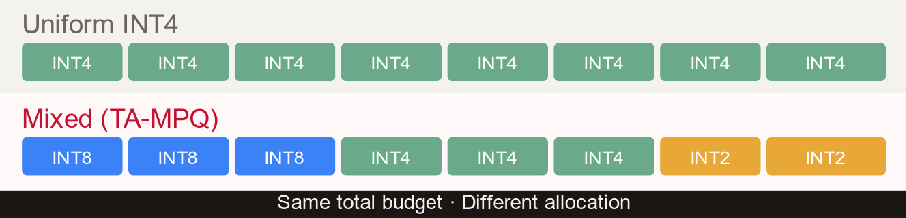
\includegraphics[width=0.78\textwidth]{figures/poster_budget_allocation.pdf}
\caption{Budget-preserving precision reallocation. Uniform \intfour{} assigns the same precision everywhere, while \method{} promotes selected high-sensitivity groups to \inteight{} and offsets the extra raw-bit cost with selected \inttwo{} demotions.}
\label{fig:budget-allocation}
\end{figure*}

\section{Related Work}

\paragraph{Post-training quantization for LLMs.}
Post-training quantization compresses a pretrained model without retraining the full model. LLM.int8() showed that transformer inference can be made practical at 8-bit precision by treating outlier dimensions carefully \cite{dettmers2022llmint8}. GPTQ frames large transformer compression as one-shot weight quantization and reports reducing weights to ``3 or 4 bits per weight'' with limited degradation \cite{frantar2023gptq}. SmoothQuant shifts quantization difficulty from activations to weights through an equivalent smoothing transformation \cite{xiao2023smoothquant}. These methods establish that low-bit post-training quantization can preserve useful behavior, but they mostly answer how to quantize under a chosen recipe rather than how to choose task-specific bit-width assignments under a strict footprint.

\paragraph{Activation-aware and task-aware quantization.}
Activation-aware methods use calibration signals to decide which values are important to preserve. AWQ protects salient weights using activation observations and explicitly states that ``protecting 1\% of salient weights'' can reduce quantization error \cite{lin2024awq}. You Had One Job extends this direction toward per-task mixed precision by using task-conditioned signals from hidden representations and sensitivity tests \cite{levi2026youhadonejob}. \method{} uses the same broad principle as a profiler but differs in the search objective: every candidate must remain at or below the raw footprint of uniform \intfour{}.

\paragraph{Mixed precision as budgeted allocation.}
Mixed-precision quantization treats bit-widths as allocation decisions rather than as a model-wide setting. This is a natural fit for transformers because attention projections, MLP projections, and output heads are not equally important for every workload. The difficulty is that the search space is combinatorial and the budget is discrete. \method{} deliberately narrows this search to an ordered frontier so that each evaluated policy is feasible, interpretable, and reproducible.

\paragraph{Evaluation tasks for reasoning and coding.}
The final evaluation suite covers both recognition-style and generation-style tasks. MMLU measures broad multitask understanding through multiple-choice questions across many domains \cite{hendrycks2021mmlu}; the MMLU-coding slice used here preserves that recognition-style format while focusing on coding-related questions. HumanEval measures ``functional correctness for synthesizing programs from docstrings'' \cite{chen2021codex}. EvalPlus augments HumanEval with stronger tests for generated code \cite{liu2023evalplus}. BigCodeBench targets code generation with ``diverse function calls as tools'' and complex instructions \cite{zhuo2025bigcodebench}. MATH introduces ``12,500 challenging competition mathematics problems'' and is useful for reasoning-heavy evaluation \cite{hendrycks2021math}. Together, these benchmarks provide the workload diversity needed to test whether one searched coding policy transfers across multiple coding tasks and whether a separate math policy behaves differently under long-form reasoning conditions.

\section{Problem}

Let a pretrained transformer contain a set of quantizable groups
\[
G = \{g_1, g_2, \ldots, g_m\}.
\]
Each group $g$ has parameter count $n_g$ and receives a bit-width $b_g \in \{2,4,8\}$. In the current system, the grouping rule is per-block component assignment: each quantization group corresponds to one concrete linear module inside a transformer block or to a small number of special linear modules outside the repeated blocks. Examples include attention projections, MLP projections, and the language-model head.

The raw weight cost of a policy $p$ is
\[
B(p) = \sum_{g \in G} n_g b_g.
\]
The target budget is the cost of uniform \intfour{}:
\[
B_{\mathrm{INT4}} = \sum_{g \in G} 4n_g.
\]
The feasible set is therefore
\[
\mathcal{P} = \{p : B(p) \leq B_{\mathrm{INT4}}\}.
\]
This raw-bit accounting is the feasibility test for every generated policy. A policy may be under budget, but it is not accepted if its quantized weight cost exceeds the uniform-\intfour{} target.

The optimization goal is to find a policy in $\mathcal{P}$ that performs well on a target task. This is not equivalent to maximizing the number of \inteight{} groups because group sizes vary. A small group can be promoted cheaply, while a large group can consume much of the promotion budget. Likewise, a small \inttwo{} demotion may not offset an expensive \inteight{} promotion. The method must therefore reason over true parameter mass, not only group count.

\section{Overview}

\method{} converts task-aware mixed-precision search into a one-dimensional frontier over real budget-feasible policies. The pipeline has five stages. First, it enumerates quantizable linear groups and records their true parameter counts. Second, it estimates task sensitivity for each group. Third, it constructs a greedy path from uniform \intfour{} toward increasingly mixed policies. Fourth, it selects coarse and refined candidate snapshots from that path. Fifth, it quantizes and evaluates the selected policies as real artifacts.

The system takes as input a source model, a target workload, calibration prompts, and an exact raw-weight budget. It outputs a runnable mixed-precision PTQ artifact and an evaluation record for the selected policy. The implemented components are the group registry, sensitivity profiler interface, exact-budget frontier builder, and coarse-to-fine selector; final quantized artifacts are instantiated through the adopted \texttt{llmcompressor.oneshot} PTQ backend.

\begin{figure*}[t]
\centering
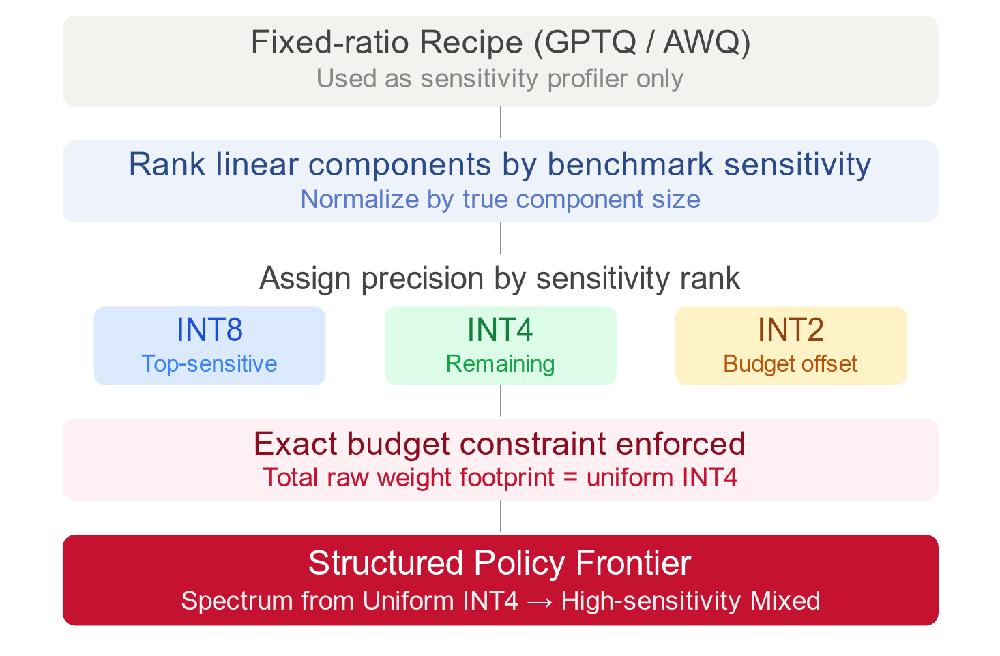
\includegraphics[width=0.64\textwidth]{figures/poster_method_pipeline.pdf}
\caption{High-level \method{} pipeline. Fixed-ratio quantization recipes are used only to obtain task sensitivity signals; the search then ranks groups by sensitivity per true bit cost, assigns \inteight{}, \intfour{}, and \inttwo{} under an exact raw-footprint constraint, and produces a structured policy frontier.}
\label{fig:method-pipeline}
\end{figure*}

\section{Method}

\subsection{Group Registry}

The atomic search unit is a quantization group, not an entire transformer block. Under per-block component grouping, every group records a block index when applicable, a component type, a parameter count, and whether it may be quantized. This design keeps the search interpretable: a selected policy can be reported as assignments over components such as attention projections and MLP projections, rather than as an opaque vector of bits.

This granularity is a compromise. Whole-block assignment would be easier to serve and explain, but it is too coarse to distinguish attention and MLP submodules. Tensor-level assignment would be more flexible but would increase the search space and make policy interpretation harder. Per-block component grouping keeps the search space small enough for frontier construction while preserving meaningful transformer structure.

\subsection{Task Sensitivity Profiling}

The task sensitivity profiler is TAQ-KL-lite. It loads the model in BF16, prepares calibration prompts from the target task, records baseline next-token logits, and estimates how much a group-level perturbation changes the output distribution. For each group and candidate bit-width, the profiler injects quantization-shaped noise at that group's linear module and computes KL divergence between the baseline and perturbed next-token distributions.

The profiler exports three quantities used by the frontier builder. The first is the estimated perturbation risk at \intfour{}. The second is the nonnegative drop in risk from moving a group from \intfour{} to \inteight{}. The third is the nonnegative increase in risk from moving a group from \intfour{} to \inttwo{}. The frontier builder uses the improvement from \intfour{} to \inteight{} as promotion value and the degradation from \intfour{} to \inttwo{} as demotion cost.

\subsection{Greedy Exact-Budget Path}

The greedy path starts with every quantizable group at \intfour{}. Candidate promotions are sorted by promotion value divided by the true extra bit cost $4n_g$. This makes promotion priority size-aware: a group must justify its precision increase relative to the number of additional bits it consumes.

When a trial promotion would exceed the target budget, the method searches for compensating demotions. It considers groups still at \intfour{}, excludes the group being promoted, filters out groups with minimum-bit constraints, and ranks demotion candidates by demotion cost per saved bit. It then runs a local beam subset-cover procedure: each beam state tracks saved bits, accumulated demotion cost, and chosen groups; states with remaining shortfall are ranked behind states that cover the deficit; covered states are ranked by demotion cost plus an overshoot penalty. If the repaired trial policy is feasible, it becomes the next path state.

This path is intentionally monotone in construction but not monotone in expected accuracy. Moving along the path generally means adding more \inteight{} mass and the required \inttwo{} compensation. Accuracy can rise or fall because each step changes multiple groups. The path is useful because it is real, deterministic, deduplicated by policy identity, and budget-feasible at every accepted step.

\subsection{Coarse-to-Fine Selection}

Coarse candidates are selected from the realized path itself. The selector deduplicates the path, removes the uniform \intfour{} anchor, removes the greedy max-\inteight{} endpoint, and places evenly spaced target points over the realized \inteight{} parameter-mass fraction of the remaining path. Each target is snapped to the nearest unused policy. Ties are resolved by lower realized \inttwo{} mass, earlier path index, and finally policy identity.

\begin{figure}[t]
\centering
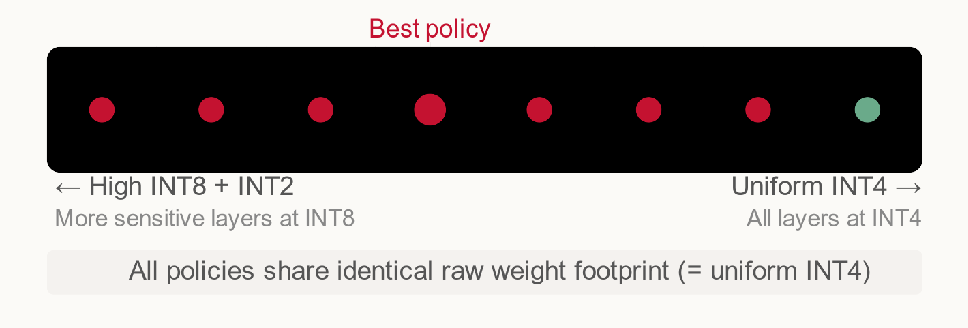
\includegraphics[width=0.98\columnwidth]{figures/poster_policy_frontier.pdf}
\caption{Coarse selection over the realized policy frontier. The search divides the frontier into sectors over realized \inteight{} parameter-mass fraction and evaluates real path snapshots rather than constructing candidates from requested percentages.}
\label{fig:policy-frontier}
\end{figure}

Refinement is local on the same greedy path. The selector first chooses the best coarse policy after applying the configured accuracy tie band and tie-break rules. Optionally, it may include a second seed if that seed is within the allowed correct-answer gap, sufficiently separated in realized \inteight{} mass, and distinct by policy identity. Around each seed path index, the method builds a local window and selects evenly spaced unused policies.

\begin{table}[t]
\caption{Algorithmic objects used by \method{}. The table describes the paper-level algorithmic object rather than experiment entrypoints.}
\label{tab:algorithmic-objects}
\centering
\begin{tabular}{p{0.30\columnwidth}p{0.60\columnwidth}}
\toprule
Object & Role \\
\midrule
Quantization group & Atomic policy unit with bit-width, parameter count, component label, and quantizability flag. \\
Raw \intfour{} budget & Feasibility constraint equal to assigning every quantizable group to \intfour{}. \\
Sensitivity score & KL-based estimate of how much precision changes perturb target-task next-token distributions. \\
Greedy path state & Unique budget-feasible assignment produced by one accepted promotion plus any required demotions. \\
Coarse/refine candidate & Real path snapshot selected by realized \inteight{} mass, not by requested percentage. \\
\bottomrule
\end{tabular}
\end{table}

\section{Evaluation}

\subsection{Experimental Setup}

\paragraph{Model and grouping.}
The active model is Qwen3.5-9B. The active bit space is \{\inttwo{}, \intfour{}, \inteight{}\}. The active group granularity is per-block component grouping. The budget is raw weight footprint less than or equal to uniform \intfour{}. The language-model head is kept at least at \intfour{} as a minimum-bit constraint.

\paragraph{Search splits.}
The staged search has three evaluation phases. The coarse phase evaluates eight interior path snapshots on a shared question set. The refine phase evaluates four local path snapshots around the winning coarse region on a larger and disjoint question set. The final phase evaluates the selected winner on the held-out split. The uniform \intfour{} anchor is treated as a baseline rather than as a coarse candidate, and the greedy max-\inteight{} endpoint is diagnostic rather than part of coarse search.

\paragraph{Baselines and metrics.}
The reported results compare the selected mixed policy against BF16, uniform \inteight{}, and uniform \intfour{} baselines under the same task protocol. For classification-style and math tasks, the tables report accuracy, correct count, token-limit hit count, average completion tokens, median completion tokens, p95 completion tokens, average latency, median latency, and p95 latency where applicable. For code-generation tasks, the report emphasizes pass@1, execution status, capped-generation counts, and completion-token statistics.

\paragraph{Quantization path.}
All quantized artifacts in the current study are instantiated with the same \texttt{llmcompressor.oneshot} post-training quantization pipeline. This choice keeps the backend fixed across mixed, uniform \inteight{}, and uniform \intfour{} runs so that the main experimental question remains allocation-focused: whether exact-budget bit reassignment improves task performance under a common quantization path. Stronger weight-reconstruction methods such as GPTQ \cite{frantar2023gptq} and AWQ \cite{lin2024awq} are intentionally not used as the primary artifact path in this report, because doing so would entangle the effect of workload-aware allocation with the effect of per-weight refinement. Instead, GPTQ/AWQ are treated as compatible future extensions that could be layered on top of the current allocation policy.

\paragraph{Prompting protocols.}
Prompting follows the native or currently supported protocol for each benchmark. MMLU-coding and MATH-500 use the simple-evals harness and prompt format \cite{openai_simple_evals}, with CoT enabled for MMLU-coding and a non-thinking prompt for MATH-500. HumanEval and HumanEval+ use the EvalPlus code-generation harness \cite{liu2023evalplus}, and BigCodeBench-Hard uses its official instruct-style code-generation prompt \cite{zhuo2025bigcodebench}.

\paragraph{Serving caveat.}
Latency should be interpreted carefully because the current artifact path uses one-shot post-training quantization artifacts rather than an optimized mixed-precision serving stack. Accuracy and token usage are therefore stronger signals than raw latency at this stage.

\subsection{Results}
\label{sec:results}

This section reports workload-family-specific results under the exact raw weight footprint of uniform \intfour{}. The mixed coding policy is \texttt{gpf\_refine\_00\_i0112} (hash \texttt{7caae6e48fce...2043e4}), searched on MMLU-coding and then transferred unchanged to HumanEval, HumanEval+, and BigCodeBench-Hard. The mixed math policy is \texttt{gpf\_refine\_02\_i0110} (hash \texttt{9bbaf3a7d0e0...59b9e9}), searched for MATH-500 and then evaluated under two token-wall settings. All reported numbers use greedy decoding on held-out evaluation slices with benchmark-specific prompt protocols. Across the evaluated benchmarks, exact-budget mixed precision reliably improves over uniform \intfour{}, but it does not surpass stronger higher-precision baselines overall, including uniform \inteight{} and BF16.

\subsubsection{Frozen Policies and Evaluation Protocol}

Table~\ref{tab:results-artifact-registry} ties the main empirical claims to explicit policy identifiers and evaluation settings. For the coding route, all reported gains come from a single mixed policy transferred across multiple coding benchmarks. For the math route, all reported gains come from one MATH-oriented policy evaluated twice with different token walls.

\begin{table*}[t]
\centering
\caption{Mixed-policy registry. The coding policy is reused unchanged across all coding benchmarks; the math policy is reused unchanged across both MATH-500 token-wall settings.}
\label{tab:results-artifact-registry}
\footnotesize
\begin{tabular}{p{0.12\textwidth}p{0.18\textwidth}p{0.14\textwidth}p{0.18\textwidth}p{0.26\textwidth}}
\toprule
Workload family & Policy identifier & Search task & Held-out evaluation slice & Protocol summary \\
\midrule
Coding & \texttt{gpf\_refine\_00\_i0112} & MMLU-coding & MMLU-coding last100; full HumanEval / HumanEval+; full BigCodeBench-Hard & Greedy decoding. MMLU-coding uses simple-evals CoT with \texttt{max\_new\_tokens}=4096; HumanEval / HumanEval+ use EvalPlus with \texttt{max\_new\_tokens}=768; BigCodeBench-Hard uses the official instruct prompt with \texttt{max\_new\_tokens}=1280. \\
\midrule
Math & \texttt{gpf\_refine\_02\_i0110} & MATH-500 & MATH-500 last100 at \texttt{max\_new\_tokens}=4096 and 20000 & Greedy decoding with the simple-evals non-thinking prompt under two token-wall settings. \\
\bottomrule
\end{tabular}
\end{table*}

\subsubsection{Main Quantitative Results}

Table~\ref{tab:results-main-summary} gives the headline benchmark scores. The mixed coding policy is a clear improvement over uniform \intfour{} on generative coding benchmarks, but not on multiple-choice coding. The mixed math policy improves over uniform \intfour{} under both MATH token-wall settings, although uniform \inteight{} remains the strongest baseline on that task.

\begin{table*}[t]
\centering
\caption{Main benchmark outcomes under frozen evaluation settings. HumanEval and HumanEval+ share the same generated samples and therefore differ only in the execution-based scoring harness.}
\label{tab:results-main-summary}
\footnotesize
\begin{tabular}{llrrrr}
\toprule
Benchmark & Metric & BF16 & Uniform \inteight{} & Uniform \intfour{} & Mixed \\
\midrule
MMLU-coding last100 & Accuracy & 95.0\% & 94.0\% & 91.0\% & 91.0\% \\
HumanEval & Pass@1 & 87.8\% & 89.0\% & 81.1\% & 84.8\% \\
HumanEval+ & Pass@1 & 82.3\% & 82.3\% & 76.8\% & 79.9\% \\
BigCodeBench-Hard & Pass@1 & 29.05\% & 27.03\% & 16.89\% & 23.65\% \\
BigCodeBench-Hard & Passed tasks & 43/148 & 40/148 & 25/148 & 35/148 \\
MATH-500 @4096 & Accuracy & 86.0\% & 88.0\% & 80.0\% & 84.0\% \\
MATH-500 @20000 & Accuracy & 87.0\% & 91.0\% & 86.0\% & 89.0\% \\
\bottomrule
\end{tabular}
\end{table*}

The coding results split cleanly into one no-gain case and several positive cases. On MMLU-coding last100, the mixed coding policy reaches 91.0\% accuracy, exactly matching uniform \intfour{} rather than improving over it. MMLU-coding therefore functions as a negative or inconclusive case for mixed-over-\intfour{} gains. The current evidence does not support a claim that the mixed policy helps uniformly across all coding benchmarks.

The picture is more favorable on generative coding tasks. On HumanEval, mixed improves pass@1 from 81.1\% to 84.8\% relative to uniform \intfour{}, recovering 3.7 points. On HumanEval+, the gain is 3.1 points, from 76.8\% to 79.9\%. BigCodeBench-Hard provides the clearest current coding result: uniform \intfour{} passes only 25 of 148 tasks, while the mixed policy passes 35 of 148. Relative to BF16, which passes 43 tasks, the mixed policy recovers 10 of the 18 tasks lost by uniform \intfour{}. Taken together, these results suggest that the benefit of task-aware precision reallocation is easier to observe on generative synthesis than on multiple-choice recognition.

\subsubsection{MATH-500 and Token-Wall Sensitivity}

The MATH results need to be interpreted jointly with the generation budget. Table~\ref{tab:results-math-tokenwall} expands the score comparison to include token-wall hit counts and completion-length statistics for both the 4096-token and 20000-token settings. The 4096-token setting is a realistic but restrictive wall; the 20000-token setting is a diagnostic run intended to separate genuine quantization degradation from truncation-induced failures.

\begin{table*}[t]
\centering
\caption{MATH-500 last100 under two token walls. Both runs use the same held-out last100 slice, greedy decoding, and the simple-evals non-thinking prompt; only \texttt{max\_new\_tokens} changes.}
\label{tab:results-math-tokenwall}
\footnotesize
\begin{tabular}{llrrrr}
\toprule
Setting & Metric & BF16 & Uniform \inteight{} & Uniform \intfour{} & Mixed \\
\midrule
MATH-500 @4096 & Accuracy & 86.0\% & 88.0\% & 80.0\% & 84.0\% \\
MATH-500 @4096 & Correct & 86/100 & 88/100 & 80/100 & 84/100 \\
MATH-500 @4096 & Token-wall hits & 7 & 6 & 14 & 7 \\
MATH-500 @4096 & Avg.\ completion tokens & 1167.0 & 1168.5 & 1494.3 & 1284.5 \\
MATH-500 @4096 & P95 completion tokens & 4096.0 & 4096.0 & 4096.0 & 4096.0 \\
\midrule
MATH-500 @20000 & Accuracy & 87.0\% & 91.0\% & 86.0\% & 89.0\% \\
MATH-500 @20000 & Correct & 87/100 & 91/100 & 86/100 & 89/100 \\
MATH-500 @20000 & Token-wall hits & 2 & 2 & 7 & 6 \\
MATH-500 @20000 & Avg.\ completion tokens & 1663.7 & 1654.0 & 3002.2 & 2349.4 \\
MATH-500 @20000 & P95 completion tokens & 6558.2 & 4332.8 & 20000.0 & 20000.0 \\
\bottomrule
\end{tabular}
\end{table*}

Several conclusions follow from Table~\ref{tab:results-math-tokenwall}. First, all four models improve when the token wall is relaxed, so the tighter 4096-token setting is not merely a harmless formatting choice. Second, the improvements are larger for lower-precision models: BF16 rises by 1 point from 86 to 87, uniform \inteight{} rises by 3 points from 88 to 91, uniform \intfour{} rises by 6 points from 80 to 86, and the mixed math policy rises by 5 points from 84 to 89. Third, the token-wall hit counts follow the same trend: the lower-precision models are capped more often, especially under the tighter wall. This indicates that part of the gap observed on MATH-500 under \texttt{max\_new\_tokens}=4096 is due to truncation rather than quantization error alone.

The ranking under the 20000-token diagnostic run is also instructive. Uniform \inteight{} is the strongest baseline at 91.0\%, the mixed math policy follows at 89.0\%, BF16 reaches 87.0\%, and uniform \intfour{} reaches 86.0\%. This ordering should not be read as evidence that low-bit models are inherently better than the native model. A safer interpretation is that, under this particular prompt, parser, and greedy decoding protocol, widening the token budget changes which models are most often truncated before landing on a correct boxed answer. MATH-500 is therefore a task where token-wall control is inseparable from quantization interpretation.

\subsubsection{Completion-Token Usage Across the Suite}

Accuracy is the primary metric, but completion-token usage gives a second and surprisingly consistent view of model behavior. Table~\ref{tab:results-token-summary} shows that the mixed policy uses fewer completion tokens than uniform \intfour{} on every benchmark in the evaluated suite. This pattern holds on MMLU-coding, HumanEval, BigCodeBench-Hard, and both MATH settings.

\begin{table*}[t]
\centering
\caption{Completion-token usage under the same frozen evaluation settings as the main benchmark tables. HumanEval and HumanEval+ share the same generations and therefore the same token statistics.}
\label{tab:results-token-summary}
\footnotesize
\begin{tabular}{lrrrr}
\toprule
Benchmark & BF16 & Uniform \inteight{} & Uniform \intfour{} & Mixed \\
\midrule
MMLU-coding last100 (avg completion tokens) & 647.8 & 696.5 & 903.8 & 787.4 \\
MMLU-coding last100 (p95 completion tokens) & 1702.3 & 1446.4 & 2562.7 & 1869.1 \\
\midrule
HumanEval / HumanEval+ (avg completion tokens) & 360.8 & 364.8 & 412.2 & 358.9 \\
HumanEval / HumanEval+ (p95 completion tokens) & 768.0 & 768.0 & 768.0 & 759.4 \\
\midrule
BigCodeBench-Hard (avg completion tokens) & 512.2 & 511.0 & 533.7 & 501.7 \\
BigCodeBench-Hard (p95 completion tokens) & 896.1 & 918.7 & 933.7 & 872.6 \\
\midrule
MATH-500 @4096 (avg completion tokens) & 1167.0 & 1168.5 & 1494.3 & 1284.5 \\
MATH-500 @4096 (p95 completion tokens) & 4096.0 & 4096.0 & 4096.0 & 4096.0 \\
\midrule
MATH-500 @20000 (avg completion tokens) & 1663.7 & 1654.0 & 3002.2 & 2349.4 \\
MATH-500 @20000 (p95 completion tokens) & 6558.2 & 4332.8 & 20000.0 & 20000.0 \\
\bottomrule
\end{tabular}
\end{table*}

This token pattern matters because the mixed policy often improves quality while using fewer tokens, rather than improving quality by simply generating longer outputs. On BigCodeBench-Hard, for example, mixed passes 10 more tasks than uniform \intfour{} while also using fewer average completion tokens (501.7 versus 533.7). On MATH-500 under the 20000-token wall, the mixed math policy remains substantially more token-efficient than uniform \intfour{} (2349.4 versus 3002.2) while also being 3 points more accurate. A plausible interpretation is that preserving higher precision on task-sensitive groups helps keep reasoning or code generation more on-track, although this remains a hypothesis rather than a proven causal mechanism.

\subsubsection{Interpretation, Failure Cases, and Remaining Ablations}

The evidence supports a narrow but defensible claim: structured exact-budget mixed precision is a practical improvement over uniform \intfour{} under the same raw weight budget, and the clearest gains appear on generative coding benchmarks and on long-form reasoning tasks where uniform \intfour{} is especially vulnerable to truncation or drift. At the same time, the data show that mixed precision does not surpass \inteight{} or BF16 as the overall quality ceiling. Uniform \inteight{} remains the strongest baseline on MATH-500 in both token-budget settings, and MMLU-coding remains a case where mixed does not separate from uniform \intfour{}.

Several ablation axes remain important for interpreting these results: the task-sensitivity profiler, the exact-budget demotion repair rule, path-based coarse selection, and local refinement. Two of these comparisons are already partially exposed by the current numbers. First, the MATH-500 4096-versus-20000 comparison makes token-wall control explicit rather than hidden. Second, the MMLU-coding result serves as a direct no-gain case. The remaining ablations still need frozen numeric comparisons, but the present results already establish the main empirical boundary: workload-aware reallocation can recover a meaningful fraction of the quality lost by uniform \intfour{}, yet its gains are benchmark-dependent and must be interpreted alongside prompting protocol and generation-budget effects.

Finally, these results should still be read as engineering evidence rather than as high-power statistical claims. MMLU-coding and MATH-500 last100 each evaluate 100 held-out examples, HumanEval and HumanEval+ use 164 tasks, and BigCodeBench-Hard uses 148 tasks. Small margins should therefore be interpreted carefully, and future versions of this evaluation would be stronger with uncertainty estimates or paired tests where per-example outputs are available.


\section{Limitations}

The current method depends on the quality of the task sensitivity profiler. TAQ-KL-lite is a proxy: it measures output-distribution sensitivity under injected perturbations, not the exact downstream accuracy effect of assigning a group to a bit-width. This makes it useful for ranking, but not a proof that the best proxy group is always the best real promotion.

The search is structured rather than exhaustive. By constraining candidates to a greedy path, \method{} gains interpretability and budget stability, but it can miss policies that require non-greedy combinations of promotions and demotions. The method is therefore best described as a practical exact-budget frontier search, not as a global optimizer over all \inttwo{}/\intfour{}/\inteight{} assignments.

The current benchmark sizes for coarse and refine selection are modest. This makes tie handling and disjoint question sets important, but it also means small accuracy differences should not be overclaimed. The reported results should therefore be read with sampling sensitivity in mind, and uncertainty estimates or paired tests would further strengthen the evaluation.

The current serving stack is not an optimized production mixed-precision runtime. Raw footprint equality controls one important variable, but it does not guarantee equal throughput, equal peak VRAM, or equal kernel efficiency. A production claim would require an optimized \intfour{}/\inttwo{}/\inteight{} serving backend or controlled comparisons against a strong \intfour{} runtime.

The current report also isolates bit allocation from within-bit weight refinement. Because all quantized artifacts are generated through a common \texttt{llmcompressor.oneshot} path, the present results should be read as evidence about allocation quality under a fixed PTQ backend, not as an upper bound on what the same policies could achieve when combined with GPTQ or AWQ reconstruction.

The current quantization granularity is also difficult for real serving systems. Per-block component assignments are useful for search because they expose meaningful structure inside each transformer block, but they can create many small precision boundaries across attention and MLP projections. Future work should evaluate coarser granularities, such as whole-block, attention-versus-MLP, or shared-pattern grouping, to test whether most of the task-aware benefit can be preserved with policies that are easier to serve efficiently.

\section{Conclusion}

This paper frames task-aware mixed-precision quantization as exact-budget policy construction. The key idea is to spend \inteight{} precision where a task-sensitive profiler predicts high value, pay for it with low-risk \inttwo{} demotions, and search over real path snapshots rather than requested percentages. The empirical results show that this structured exact-budget route consistently improves over uniform \intfour{} on several generative coding and math benchmarks while leaving multiple-choice coding as an explicit no-gain case. The resulting picture is promising but bounded: workload-aware reallocation helps recover a meaningful portion of the quality lost by uniform \intfour{}, yet it does not currently displace stronger \inteight{} or BF16 baselines as the overall quality ceiling.

\begin{thebibliography}{9}

\bibitem[Dettmers et~al.(2022)Dettmers, Lewis, Belkada, and Zettlemoyer]{dettmers2022llmint8}
Tim Dettmers, Mike Lewis, Younes Belkada, and Luke Zettlemoyer.
\newblock LLM.int8(): 8-bit Matrix Multiplication for Transformers at Scale.
\newblock NeurIPS 2022. \url{https://arxiv.org/abs/2208.07339}.

\bibitem[Frantar et~al.(2023)Frantar, Ashkboos, Hoefler, and Alistarh]{frantar2023gptq}
Elias Frantar, Saleh Ashkboos, Torsten Hoefler, and Dan Alistarh.
\newblock GPTQ: Accurate Post-Training Quantization for Generative Pre-trained Transformers.
\newblock ICLR 2023. \url{https://arxiv.org/abs/2210.17323}.

\bibitem[Xiao et~al.(2023)Xiao, Lin, Seznec, Wu, Demouth, and Han]{xiao2023smoothquant}
Guangxuan Xiao, Ji Lin, Mickael Seznec, Hao Wu, Julien Demouth, and Song Han.
\newblock SmoothQuant: Accurate and Efficient Post-Training Quantization for Large Language Models.
\newblock ICML 2023. \url{https://proceedings.mlr.press/v202/xiao23c.html}.

\bibitem[Lin et~al.(2024)Lin, Tang, Tang, Yang, Chen, Wang, Xiao, Dang, Gan, and Han]{lin2024awq}
Ji Lin, Jiaming Tang, Haotian Tang, Shang Yang, Wei-Ming Chen, Wei-Chen Wang, Guangxuan Xiao, Xingyu Dang, Chuang Gan, and Song Han.
\newblock AWQ: Activation-aware Weight Quantization for On-Device LLM Compression and Acceleration.
\newblock MLSys 2024. \url{https://mlsys.org/virtual/2024/poster/2653}.

\bibitem[LeVi et~al.(2026)LeVi, Lapid, Himelstein, Baskin, Shwartz Ziv, and Mendelson]{levi2026youhadonejob}
Amit LeVi, Raz Lapid, Rom Himelstein, Chaim Baskin, Ravid Shwartz Ziv, and Avi Mendelson.
\newblock You Had One Job: Per-Task Quantization Using LLMs' Hidden Representations.
\newblock arXiv 2026. \url{https://arxiv.org/abs/2511.06516}.

\bibitem[Chen et~al.(2021)]{chen2021codex}
Mark Chen et al.
\newblock Evaluating Large Language Models Trained on Code.
\newblock arXiv 2021. \url{https://arxiv.org/abs/2107.03374}.

\bibitem[Liu et~al.(2023)Liu, Xia, Wang, and Zhang]{liu2023evalplus}
Jiawei Liu, Chunqiu Steven Xia, Yuyao Wang, and Lingming Zhang.
\newblock Is Your Code Generated by ChatGPT Really Correct? Rigorous Evaluation of Large Language Models for Code Generation.
\newblock NeurIPS 2023. \url{https://openreview.net/forum?id=1qvx610Cu7}.

\bibitem[Zhuo et~al.(2025)]{zhuo2025bigcodebench}
Terry Yue Zhuo et al.
\newblock BigCodeBench: Benchmarking Code Generation with Diverse Function Calls and Complex Instructions.
\newblock ICLR 2025. \url{https://openreview.net/forum?id=YrycTjllL0}.

\bibitem[Hendrycks et~al.(2021)Hendrycks, Burns, Kadavath, Arora, Basart, Tang, Song, and Steinhardt]{hendrycks2021math}
Dan Hendrycks, Collin Burns, Saurav Kadavath, Akul Arora, Steven Basart, Eric Tang, Dawn Song, and Jacob Steinhardt.
\newblock Measuring Mathematical Problem Solving With the MATH Dataset.
\newblock NeurIPS Datasets and Benchmarks 2021.

\bibitem[Hendrycks et~al.(2021)Hendrycks, Burns, Basart, Zou, Mazeika, Song, and Steinhardt]{hendrycks2021mmlu}
Dan Hendrycks, Collin Burns, Steven Basart, Andy Zou, Mantas Mazeika, Dawn Song, and Jacob Steinhardt.
\newblock Measuring Massive Multitask Language Understanding.
\newblock ICLR 2021. \url{https://arxiv.org/abs/2009.03300}.

\bibitem[OpenAI(2024)]{openai_simple_evals}
OpenAI.
\newblock simple-evals.
\newblock Software repository, 2024. \url{https://github.com/openai/simple-evals}.

\end{thebibliography}

\end{document}
